\documentclass[margin=5mm]{article}
\usepackage{tikz}
\usepackage{parskip}
\usepackage{listings}
\usepackage{color}
\usepackage{amsmath}


\usepackage[utf8]{inputenc}
\usepackage[english]{babel}
 \usepackage{hyperref}
\hypersetup{
    colorlinks=true,
    linkcolor=blue,
    filecolor=magenta,      
    urlcolor=cyan,
}
 
\urlstyle{same}

\usetikzlibrary{matrix,calc}
\definecolor{dkgreen}{rgb}{0,0.6,0}
\definecolor{gray}{rgb}{0.5,0.5,0.5}
\definecolor{mauve}{rgb}{0.58,0,0.82}

\lstset{frame=tb,
  aboveskip=3mm,
  belowskip=3mm,
  showstringspaces=false,
  columns=flexible,
  basicstyle={\small\ttfamily},
  numbers=none,
  numberstyle=\tiny\color{gray},
  keywordstyle=\color{blue},
  commentstyle=\color{dkgreen},
  stringstyle=\color{mauve},
  breaklines=true,
  breakatwhitespace=true,
  tabsize=3
}


\begin{document}

\section{Send Population Model}

From Simulation, Modeling and Analysis:

\begin{quote}
The state of a system is defined to be the collection of variables
necessary to describe a system at a particular point in time, relative
to the objective of a study.
\end{quote}

and

\begin{quote}
A system is defined to be the collection of entities that act and
interact towards the accomplishment of some goal.
\end{quote}

In the Send Model the collection of entities that make up the system
are drawn from $S \times N \times AY$ where $S = \{MMSIB, ISS, ISSR, \dots, MU\}$,
$N = \{CL, \dots, NONSEND\}$, $AY = \{4, \dots, 24\}$.

Each entity has a single state variable $T$ which represents its total
population.

The points in time for which we can examine an entity's state is per
calendar year.

The Send simulation uses the population of each of the system 
entities (population state) for one calendar year to predict the
population state of the next calendar year.

By visualising the mathematical structures that govern population
state we can gain an intuitive understanding of how the model works.

In Fig.\ref{state} below $T_{s_x,n_y,ay_z}$ represents the total
population of some setting $s_x$, need $n_y$ and academic year
$ay_z$.Where $x$, $y$, $z$ are any integer index into the respective
ordered sets: $S$, $N$, $AY$.

\begin{figure}[h!]
  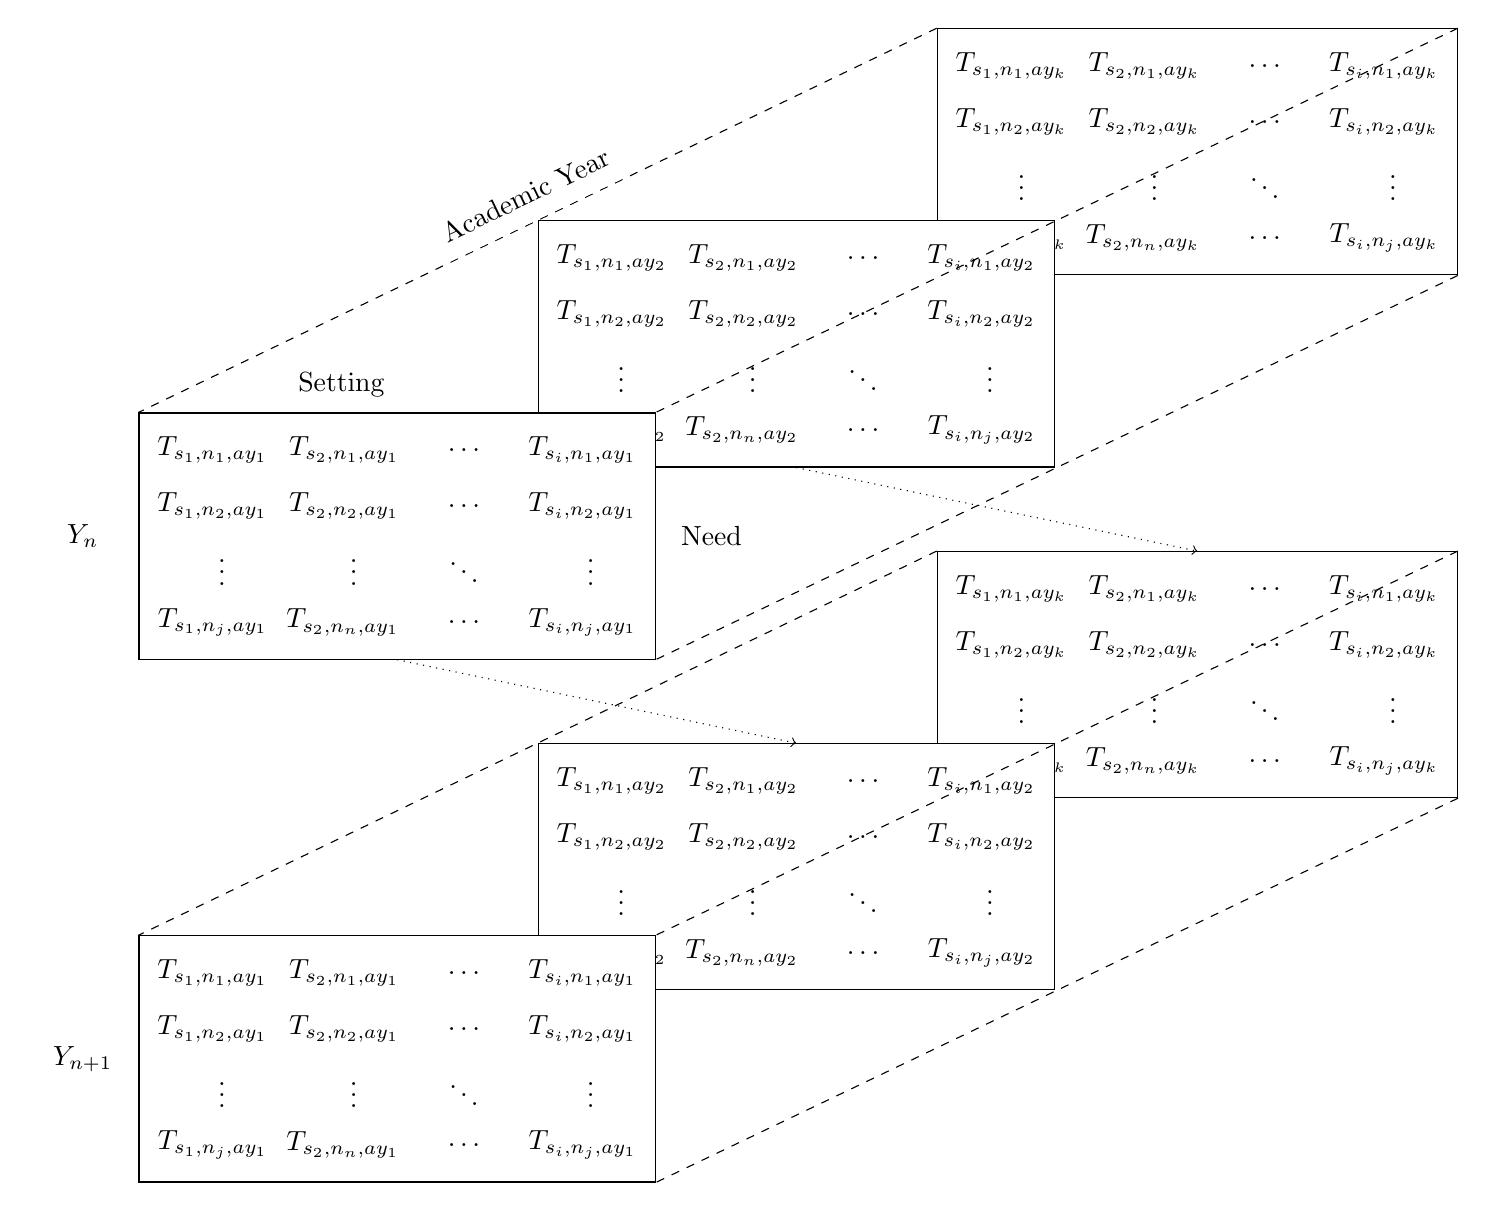
\begin{tikzpicture}[every node/.style={anchor=north
      east,fill=white,minimum width=1.4cm,minimum height=7mm}]

    \matrix (mA) [draw,matrix of math nodes]
    {
      T_{s_1,n_1,ay_k} & T_{s_2,n_1,ay_k} & \dots & T_{s_i,n_1,ay_k} \\
      T_{s_1,n_2,ay_k} & T_{s_2,n_2,ay_k} & \dots & T_{s_i,n_2,ay_k} \\
      \vdots & \vdots & \ddots & \vdots \\
      T_{s_1,n_j,ay_k} & T_{s_2,n_n,ay_k} & \dots & T_{s_i,n_j,ay_k} \\
    };

    \matrix (mB) [draw,matrix of math nodes] at ($(mA.south west)+(1.5,0.7)$)
    {
      T_{s_1,n_1,ay_2} & T_{s_2,n_1,ay_2} & \dots & T_{s_i,n_1,ay_2} \\
      T_{s_1,n_2,ay_2} & T_{s_2,n_2,ay_2} & \dots & T_{s_i,n_2,ay_2} \\
      \vdots & \vdots & \ddots & \vdots \\
      T_{s_1,n_j,ay_2} & T_{s_2,n_n,ay_2} & \dots & T_{s_i,n_j,ay_2} \\
    };

    \matrix (mC) [draw,matrix of math nodes] at ($(mB.south west)+(1.5,0.7)$)
    {
      T_{s_1,n_1,ay_1} & T_{s_2,n_1,ay_1} & \dots & T_{s_i,n_1,ay_1} \\
      T_{s_1,n_2,ay_1} & T_{s_2,n_2,ay_1} & \dots & T_{s_i,n_2,ay_1} \\
      \vdots & \vdots & \ddots & \vdots \\
      T_{s_1,n_j,ay_1} & T_{s_2,n_n,ay_1} & \dots & T_{s_i,n_j,ay_1} \\
    };

    \draw[dashed](mA.north east)--(mC.north east);
    \draw[dashed](mA.north west)-- node[sloped,above] {Academic Year} (mC.north west);
    \draw[dashed](mA.south east)--(mC.south east);

    \node [above left] at (mC.north) {Setting};
    \node [right] at (mC.east) {Need};
    \node [left] at (mC.west) {$Y_n$};

    \matrix (mD) [draw,matrix of math nodes] at ($(mA.south east)+(0,-3.5)$)
    {
      T_{s_1,n_1,ay_k} & T_{s_2,n_1,ay_k} & \dots & T_{s_i,n_1,ay_k} \\
      T_{s_1,n_2,ay_k} & T_{s_2,n_2,ay_k} & \dots & T_{s_i,n_2,ay_k} \\
      \vdots & \vdots & \ddots & \vdots \\
      T_{s_1,n_j,ay_k} & T_{s_2,n_n,ay_k} & \dots & T_{s_i,n_j,ay_k} \\
    };

    \matrix (mE) [draw,matrix of math nodes] at ($(mB.south east)+(0,-3.5)$)
    {
      T_{s_1,n_1,ay_2} & T_{s_2,n_1,ay_2} & \dots & T_{s_i,n_1,ay_2} \\
      T_{s_1,n_2,ay_2} & T_{s_2,n_2,ay_2} & \dots & T_{s_i,n_2,ay_2} \\
      \vdots & \vdots & \ddots & \vdots \\
      T_{s_1,n_j,ay_2} & T_{s_2,n_n,ay_2} & \dots & T_{s_i,n_j,ay_2} \\
    };

    \matrix (mF) [draw,matrix of math nodes] at ($(mC.south east) + (0,-3.5)$)
    {
      T_{s_1,n_1,ay_1} & T_{s_2,n_1,ay_1} & \dots & T_{s_i,n_1,ay_1} \\
      T_{s_1,n_2,ay_1} & T_{s_2,n_2,ay_1} & \dots & T_{s_i,n_2,ay_1} \\
      \vdots & \vdots & \ddots & \vdots \\
      T_{s_1,n_j,ay_1} & T_{s_2,n_n,ay_1} & \dots & T_{s_i,n_j,ay_1} \\
    };

    \draw[dashed](mD.north east)--(mF.north east);
    \draw[dashed](mD.north west)--(mF.north west);
    \draw[dashed](mD.south east)--(mF.south east);

    \draw[dotted,->](mC.south)--(mE.north);
    \draw[dotted,->](mB.south)--(mD.north);

    \node [left] at (mF.west) {$Y_{n+1}$};
  \end{tikzpicture}
  \caption{State Transitions in the Send Markov Chain\label{state}
  }
\end{figure}

\subsection{Markov Chain}

This section and the next are a detour into how a the Send model would
look if it were implemented using just Markov Chains.  If we
understand this we understand why we can see the Send Model is''
`Markov like`''.

The initial state of our Markov Chain, $Y_0$ is constructed from the
historic data provided by the client (we simply count the number of
pupils that appear e.g for a single state index, $(s_1,n_1,ay_1)$, how
many rows in our input data match?

In Fig.\ref{state} $Y_{n+1}$ is the next state of our Markov Chain.

How we transition from $Y_{n}$ to $Y_{n+1}$ is the subject of the next
section.  However, it's worth noting now that the dotted arrows on the
diagram represent how the $T$'s of one academic year transition into
the next academic year, in the following calendar year.

The complete state of the model is represented as $S = \{Y_0, \dots,
Y_n\}$ where $n$ is the number of years we run the simulation for.

\subsection{Markov Transition Matrix}

This section can be skipped - it explores what Markov Transition
Matrix would look like if the model used it.

In mathematics a Markov Transition Matrix is formally a matrix
containing the probability of transitioning between Markov
states. \textit{Do not confuse the Markov Transition (Probability)
  Matrix with the Send Model's Transitions data file.}  Conceptually,
for the Send Model, it can be thought of as telling us what percentage
of $T_{s_x,n_y,ay_z}$ will move to another state \- for each of the
valid (allowed) states that $T_{s_x,n_y,ay_z}$ can move to.  Sometimes
this is referred to as \textit{rates}.

By looking at the historic data we could work out the expectation of
each of our transitions and build this matrix.  We visualise what this
looks like in Fig.\ref{transition matrix}.
\begin{figure}[h!]
  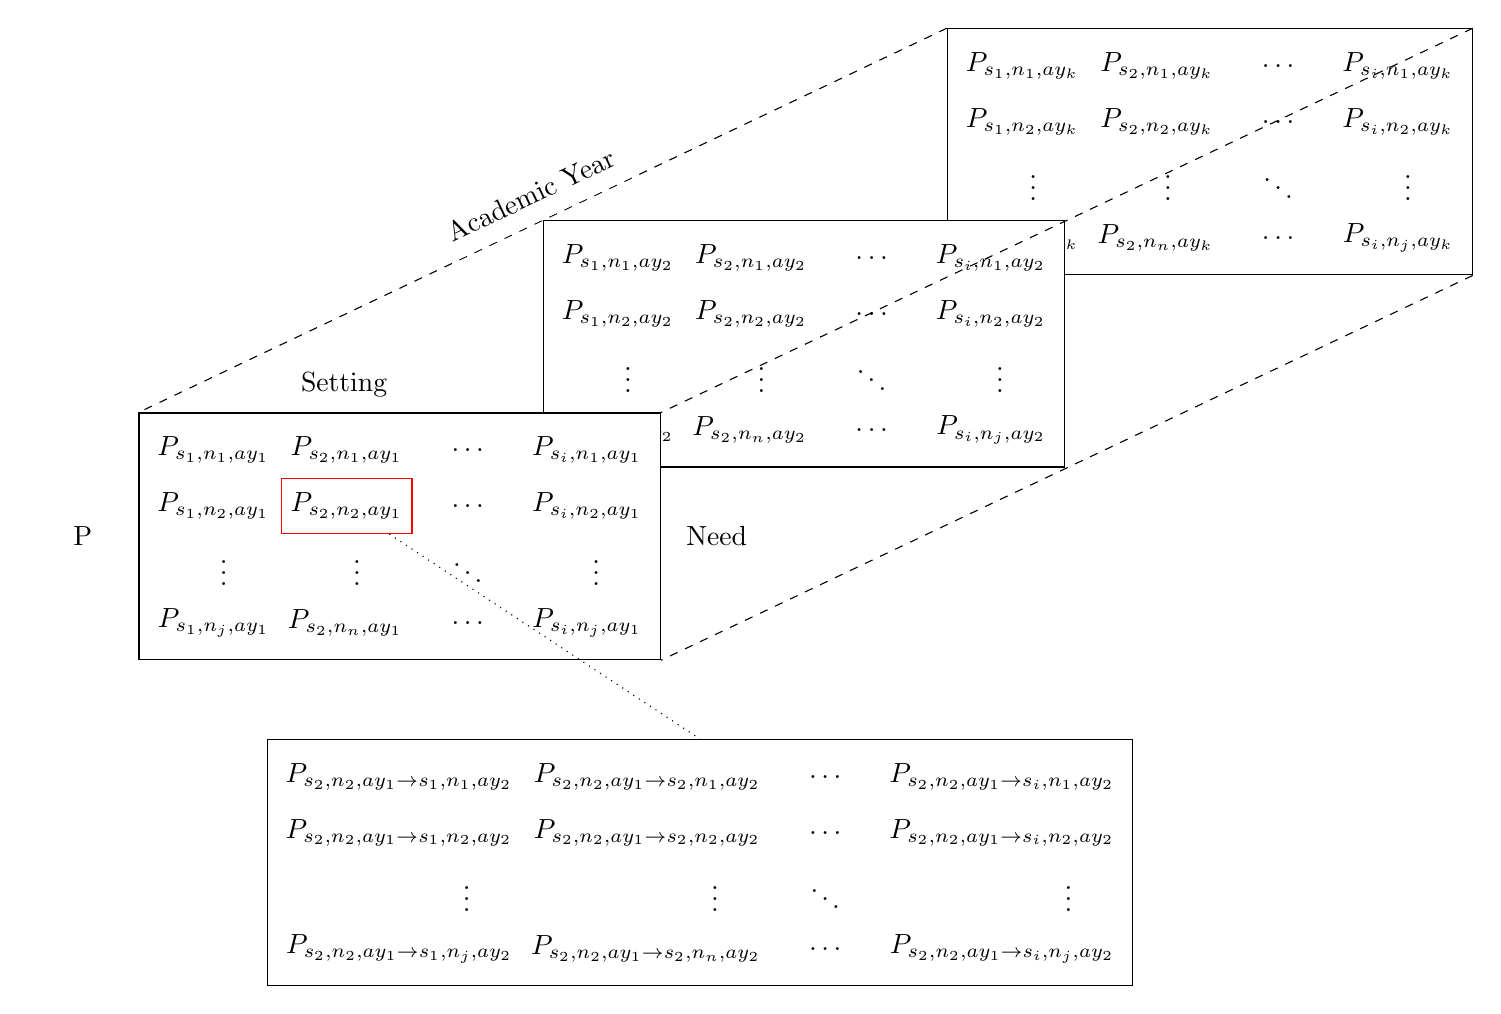
\begin{tikzpicture}[every node/.style={anchor=north east,fill=white,minimum width=1.4cm,minimum height=7mm}]

    \matrix (mA) [draw,matrix of math nodes]
    {
      P_{s_1,n_1,ay_k} & P_{s_2,n_1,ay_k} & \dots & P_{s_i,n_1,ay_k} \\
      P_{s_1,n_2,ay_k} & P_{s_2,n_2,ay_k} & \dots & P_{s_i,n_2,ay_k} \\
      \vdots & \vdots & \ddots & \vdots \\
      P_{s_1,n_j,ay_k} & P_{s_2,n_n,ay_k} & \dots & P_{s_i,n_j,ay_k} \\
    };

    \matrix (mB) [draw,matrix of math nodes] at ($(mA.south west)+(1.5,0.7)$)
    {
      P_{s_1,n_1,ay_2} & P_{s_2,n_1,ay_2} & \dots & P_{s_i,n_1,ay_2} \\
      P_{s_1,n_2,ay_2} & P_{s_2,n_2,ay_2} & \dots & P_{s_i,n_2,ay_2} \\
      \vdots & \vdots & \ddots & \vdots \\
      P_{s_1,n_j,ay_2} & P_{s_2,n_n,ay_2} & \dots & P_{s_i,n_j,ay_2} \\
    };

    \matrix (mC) [draw,matrix of math nodes] at ($(mB.south west)+(1.5,0.7)$)
    {
      P_{s_1,n_1,ay_1} & P_{s_2,n_1,ay_1} & \dots & P_{s_i,n_1,ay_1} \\
      P_{s_1,n_2,ay_1} & |[draw=red]|P_{s_2,n_2,ay_1} & \dots & P_{s_i,n_2,ay_1} \\
      \vdots & \vdots & \ddots & \vdots \\
      P_{s_1,n_j,ay_1} & P_{s_2,n_n,ay_1} & \dots & P_{s_i,n_j,ay_1} \\
    };

    \draw[dashed](mA.north east)--(mC.north east);
    \draw[dashed](mA.north west)-- node[sloped,above] {Academic Year} (mC.north west);
    \draw[dashed](mA.south east)--(mC.south east);

    \node [above left] at (mC.north) {Setting};
    \node [right] at (mC.east) {Need};
    \node [left] at (mC.west) {P};

    \matrix (mD) [draw,matrix of math nodes] at ($(mC.south east)+(6,-1)$)
    {
      P_{s_2,n_2,ay_1 \rightarrow s_1,n_1,ay_2} & P_{s_2,n_2,ay_1 \rightarrow s_2,n_1,ay_2} & \dots & P_{s_2,n_2,ay_1 \rightarrow s_i,n_1,ay_2} \\
      P_{s_2,n_2,ay_1 \rightarrow s_1,n_2,ay_2} & P_{s_2,n_2,ay_1 \rightarrow s_2,n_2,ay_2} & \dots & P_{s_2,n_2,ay_1 \rightarrow s_i,n_2,ay_2} \\
      \vdots & \vdots & \ddots & \vdots \\
      P_{s_2,n_2,ay_1 \rightarrow s_1,n_j,ay_2} & P_{s_2,n_2,ay_1 \rightarrow s_2,n_n,ay_2} & \dots & P_{s_2,n_2,ay_1 \rightarrow s_i,n_j,ay_2} \\
    };

    \draw[dotted](mC-2-2)--(mD.north);
  \end{tikzpicture}
  \caption{Markov Transition Matrix (many nested probability
    matrices)\label{transition matrix}
  }
\end{figure}

In the Fig.\ref{transition matrix} every $P_{s_i,n_j,ak_1}$ is a
probability matrix that represents the probabilities of transitioning
to any other state in the next academic year (see the diagram's
cut-out for an example.)

Armed with $P$, this rather complicated Markov Transition Matrix, we can
apply it to the initial state

$Y_1 = Y_0 \cdot P$

In fact at this point as $P$ is time independent we can work the
populations in year $n$ by

$Y_n = Y_0 \cdot P^n$

Of note is that this equation requires no tracking of $T's$ we can simply
use the above formula to work out $Y_n$. BUT we don't do this!  Why?

The send model actually sides step the creation of a Markov Transition
Matrix and takes an algorithmic approach to calculating $Y_{n+1}$'s
population.  This is done as some of the data is perhaps too sparse,
but also the algorithmic approach allows us to introduce population
increase, priors and scenarios rather more easily than modifying $P$
directly.

As we will come to see the algorithmic approach to working out the $T$
in $Y_n$ introduces stochastic processes. Thus we introduce the need to use
Monte Carlo methods to ensure confidence in our calculations.

\subsection{Send Model's Population Prediction Algorithm}

The algorithm can be simply expressed as:

$Y_{n+1} = T(Y_n)$

$Y_n$ represents calendar year n's population state, $T$ the function
that calculates the next years population state from it.  Thus the
inner working of T is the algorithm.

Let us consider first a single entity's population $t_{s_x,n_y,ay_z}$.
How will $T$ operate on this?

\subsubsection{Movers,  Non-Movers, Leavers and Joiners}

The model introduces the concepts of movers($m$), leavers($l$), and
joiners($j$).

Let $m_{s_x,n_y,ay_z}$ be defined as all the pupils that move
\textbf{into} a particular entity from another entity.

Let $n_{s_x,n_y,ay_z}$ be defined as all the pupils that
\textbf{don't} move out of a particular entity (non-movers or
stayers).

Let $l_{s_x,n_y,ay_z}$ be defined as all the pupils that
\textbf{leave} a particular entity and out of the Send programme
completely.

Let $j_{s_x,n_y,ay_z}$ be defined as all the pupils that join
\textbf{into} a particular entity from the outside populace.


So $T(Y_n)_{s_x,n_y,ay_z} = m_{s_x,n_y,ay_z} + n_{s_x,n_y,ay_z} -
l_{s_x,n_y,ay_z} + j_{s_x,n_y,ay_z} $

Reading this equation aloud makes obvious intuitive sense.  The
question now becomes how do we calculate each of the components of
this function?

In all the following sections except where noted it is assumed that
the underlying processes governing leavers, joiners, and movers are
independent and identically distributed meaning that we can combine
historic calendar years data as one.

\subsubsection{Leavers}

From our historic data we can work out the percentages over the
calendar years of how many pupils leave a particular entity,
$(s_1,n_1,ay_1)$.  Averaging this sets our expectation e.g. for
$(s_1,n_1,ay_1)$ we may expect $40\%$ of the population to leave.

For the purposes of our simulation we do not want every run to have
exactly $40\%$ of the population leave but rather have some variance
in the size.  How these variances in the population propagate through
the simulation lets us see confidence bounds when we come to
aggregate the results of many runs of the model.

A first pass at introducing variance is to use the binomial
distribution to alter the population that leaves per run.

Continuing our example given $t_{s_1,n_1,ay_1} = 100$ and an
expectation of $40\%$ then a sample of ten values looks like so:

\begin{lstlisting}
(sample 10 (binomial {:n 100 :p 0.4}))
(46 42 31 45 43 44 48 41 41 40)
\end{lstlisting}

We can further refine the introduction of variance by noting that the
expectation percentage of leavers is stronger or weaker depending
on the amount of data we have.  Intuitively if we have lots of
observations around the number of leavers then we can be much more
confident in our expectation value.  If we have very few observations
then we are much less confident it's the correct value.

The beta distribution can be used to express the variance in our
expected leaver percentage.  The parameters for the distribution
$\alpha$, $\beta$ are simply the observed leavers and non-leavers
respectively.  Drawing from the distribution is equivalent to working
out the percentage expectation (obviously slightly changed as it's
purpose is to introduce variance in this value).  For low values of
observations there will be a wide range in the values of the expected
leavers and for high values of observations there will be a much
narrower range of expected values.

If we use the results of the Beta distribution as the probability
parameter of the Binomial distribution (composition) we form what's
called a hierarchical model.  This chaining of distributions increases
the size of variance in our model runs.

Thus we can write:

\begin{equation*}
l_{s_x,n_y,ay_z} = \text{Binomial}(t_{s_x,n_y,ay_z},
\text{Beta}(\alpha^l_{s_x,n_y,ay_z}, \beta^l_{s_x,n_y,ay_z})
\end{equation*}

where $\alpha^l_{s_x,n_y,ay_z}$ represents the count of leavers over
all historic calendar years for the entity $({s_x,n_y,ay_z})$.
Similarly $\beta^l_{s_x,n_y,ay_z}$ represents the count of all non
leavers for the same entity over all historic calendar years.
$(t_{s_x,n_y,ay_z}$ represents the populatio of the entity.

The algorithm described here is a high level overview of the
implementation by the Send code base.

\subsubsection{Joiners}

The calculation for working out an entity's joiners is split into two
parts: first the expected rate of joiners is calculated per academic
year, then this additional population is assigned a need and setting.

The sum of the joiners for a single academic year over all historic
calendar years is first calculated.  Dividing through by the number of
calendar years gives the average joiners for this particular academic
year (whether this is a sensible thing to do is up for debate: if we
assume that the underlying process is independently and identically
distributed then there is no reason to divide other than to increase
our variance by lowering our observations).

Similarly we work out the number of non-joiners by taking the
joiners away from the total population for an academic year.  Again we
divide through by the calendar years to provide the average
non-joiners for an academic year.

If we take the average joiners per academic year and divide by the
average population we get the expected percentage of joiners per
academic year.  However, like for the leavers we wish to have a
variance in this value based on our confidence of the data.  Like
before, we can apply the beta distribution to do this.

Also we once more use the binomial distribution to provide variance in
our population values once we have an expected probability from the
beta distribution.

\begin{equation*}
j_{ay_z} = \text{Binomial}(t_{ay_z}, \text{Beta}(\alpha^j_{ay_z},\beta^j_{ay_z})
\end{equation*}

where $\alpha^j_{ay_z}$ is the average joiners for $ay_z$ (from the
historic calendar years) and $\beta^j_{ay_z}$ is the average
non-joiners for $ay_z$.

The second part of the calculation is to distribute the new joiners to
appropriate needs and settings.  We count for each academic year
exactly how many joiners there are from non-send to each of the
need-settings.  The proportions of which tell us how to distribute the
joiners.  Note: this time we don't divide through by the academic
years.  Armed with these proportions we can calculate the expectation
as a percentage for each e.g $10\%$ to $(s_x,n_y,ay_z)$ and $90\%$ to
$(s_j,n_k,ay_l)$.

Again, rather then a direct calculation of the population to be
assigned to each entity we introduce variance by using the multinomial
distribution.  It performs exactly the same job as the binomial except
over multiple possible outcomes.

In a now familiar pattern, we also wish to introduce variance in the
actual percentages used to calculate the assignment.  Like before, we
want high confidence in values we have lots of observed data for and
low confidence for few observations.  The Dirichlet distribution does
this for multivariates in exactly the same way beta distribution does
for two.  We combine the two to produce another hierarchical model.

\begin{equation*}
\begin{split}
  \text{Multinomial} ( & j_{ay_{z}}, \\
  & \text{Dirichlet} (\alpha^{j}_{s_x,n_y,ay_z}, \dots,
  \alpha^{j''}_{s_{x''},n_{y''},ay_{z''}}))
\end{split}
\end{equation*}

Here the $\alpha^{j}$s represent the total number of transitions from
$non\-send$ to ${s_x,n_y,ay_z}$.

The results of the multinomial function is however a vector of the
counts of the joiners for each of the possible entities.  Thus for any
particular entity of interest we need to take the appropriate index.

\begin{equation*}
  \begin{split}
    j_{s_x,n_y,ay_z} = \bigg[\text{Multinomial}( & j_{ay_z}, \\
    & \text{Dirichlet}(\alpha^{j}_{s_x,n_y,ay_z},\alpha^{j'}_{s_{x'},n_{y'},ay_{z'}}, \dots, \alpha^{j''}_{s_{x''},n_{y''},ay_{z''}}))\bigg]_{s_x,n_y,ay_z}
  \end{split}
\end{equation*}

We can write this out in full for single entity by expanding
$j_{ay_z}$.

\begin{equation*}
  \begin{split}
j_{s_x,n_y,ay_z} = \bigg[\text{Multinomial}( & \text{Binomial}( t_{ay_z},
\text{Beta}(\alpha^j_{ay_z},\beta^j_{ay_z})), \\
& \text{Dirichlet}(\alpha^{j}_{s_x,n_y,ay_z}, \dots
, \alpha^{j''}_{s_{x''},n_{y''},ay_{z''}}))\bigg]_{s_x,n_y,ay_z}
  \end{split}
\end{equation*}

Interestingly, we can immediately see that the number of joiners to an
entity is not directly related to that entity's population state,
rather it's relation is to the total population of an academic year
and the non-send to entity transitions in the observed data.

Contrast this to the leaver calculation, which is directly related to
the entity's population size - why is the academic year population
choice a better one than an entity's population?  Perhaps it's because
it incorporates any trend in leavers across all entities in an
academic year?  If so, why wouldn't we do the same for leavers?  Are
there other reasons?

\subsubsection{Movers and Non Movers}


The base form of the calculations should be by now familiar.

\begin{equation*}
  \begin{split}
m^{partial}_{s_x,n_y,ay_z} =
\text{Multinomial}( & \text{Binomial}(t_{s_x,n_y,ay_z} - l_{s_x,n_y,ay_z}, 
 \text{Beta}(\alpha^m_{s_x,n_y,ay_z},\beta^m_{s_x,n_y,ay_z})),
\\ &  \text{Dirichlet}(\alpha^{m'}_{s_x',n_y',ay_z'}, \dots,
\alpha^{m''}_{s_{x''},n_{y''},ay_{z''}}))
\end{split}
\end{equation*}

The first thing to note is that this a partial result - which we will
come to later.

Unlike joiners, but like leavers the relationship is based on the
current entity's population count (not the academic year's population
count).  However it is slightly modified in that we take the
previously calculated leavers away for this entity (as we know they
move to non-send).

The Beta params $\alpha^m$ and $\beta^m$ are the counts of the
transitions out-of-${s_x,n_y,ay_z}$-and-into-some-other-setting and the
transitions to-itself respectively.  Unlike joiners they are not
divided through by observed calendar years.

The Dirichlet params $\alpha^{m'}$'s are the counts from the observed
data of our entity ${s_x,n_y,ay_z}$ to the other entities it can move
to ${s_x',n_y',ay_z'}$ (represented by ever increasing dashes).  As
such the vector that is the result of the multinomial has no count of
any movers to our entity ${s_x,n_y,ay_z}$.  Instead we need to
calculate $m^{partial}$ for every other entity and take from each
generated vector the index that represents the population that moves
to $m_{s_x,n_y,ay_z}$.  The sum of these is the total movers into our
entity.

\begin{equation*}
  \begin{split}
    m_{s_x,n_y,ay_z} = \sum_{j \neq x, k \neq y , l \neq ay }\bigg[
        \text{Multinomial}( & \text{Binomial}(t_{s_j,n_k,ay_l} - l_{s_j,n_k,ay_l}, 
        \text{Beta}(\alpha^m_{s_j,n_k,ay_l},\beta^m_{s_j,n_k,ay_l})),
        \\ &  \text{Dirichlet}(\alpha^{m'}_{s_j',n_k',ay_l'}, \dots,
        \alpha^{m''}_{s_{j''},n_{k''},ay_{l''}}))\bigg]_{s_x,n_y,ay_z}
\end{split}
\end{equation*}

where $j$, $k$, $l$ belong to $S$, $N$, $AY$ respectively.

As we know that non-movers for an entity stay within the entity we can
just use the beta binomial to calculate these.

\begin{equation*}
  \begin{split}
    n_{s_x,n_y,ay_z} = & t_{s_x,n_y,ay_z}
    - l_{s_x,n_y,ay_z} \\ & - \text{Binomial}(t_{s_x,n_y,ay_z} - l_{s_x,n_y,ay_z}, 
\text{Beta}(\alpha^m_{s_x,n_y,ay_z},\beta^m_{s_x,n_y,ay_z}))
\end{split}
\end{equation*}

For consistency of the model that Bionomial component of the above
equation should be the same result as when it was used to calculate
the movers.

\subsubsection{The Full Equation}

Calculate next years population T for an entity given the current
years state.

$Y_{n+1}_{s_x,n_y,ay_z} = T(Y_n)_{s_x,n_y,ay_z} = m_{s_x,n_y,ay_z} + n_{s_x,n_y,ay_z} -
l_{s_x,n_y,ay_z} + j_{s_x,n_y,ay_z} $

Where

\begin{equation*}
\begin{aligned}
& \begin{split}
    m_{s_x,n_y,ay_z} = \sum_{j \neq x, k \neq y , l \neq ay }\bigg[
        \text{Multinomial}( & \text{Binomial}(t_{s_j,n_k,ay_l} - l_{s_j,n_k,ay_l}, 
        \text{Beta}(\alpha^m_{s_j,n_k,ay_l},\beta^m_{s_j,n_k,ay_l})),
        \\ &  \text{Dirichlet}(\alpha^{m'}_{s_j',n_k',ay_l'}, \dots,
        \alpha^{m''}_{s_{j''},n_{k''},ay_{l''}}))\bigg]_{s_x,n_y,ay_z}
\end{split}\\ 
& \begin{split}
    n_{s_x,n_y,ay_z} = t_{s_x,n_y,ay_z}  - l_{s_x,n_y,ay_z} & - \text{Binomial}(t_{s_x,n_y,ay_z} - l_{s_x,n_y,ay_z}, 
    & \text{Beta}(\alpha^m_{s_x,n_y,ay_z},\beta^m_{s_x,n_y,ay_z})) 
  \end{split}\\
& \begin{split}
  l_{s_x,n_y,ay_z} =
  \text{Binomial}(t_{s_x,n_y,ay_z},\text{Beta}(\alpha^l_{s_x,n_y,ay_z},
  \beta^l_{s_x,n_y,ay_z})
\end{split}\\
& \begin{split}
j_{s_x,n_y,ay_z} = \bigg[\text{Multinomial}( & \text{Binomial}( t_{ay_z},
\text{Beta}(\alpha^j_{ay_z},\beta^j_{ay_z})), \\
& \text{Dirichlet}(\alpha^{j}_{s_x,n_y,ay_z}, \dots
, \alpha^{j''}_{s_{x''},n_{y''},ay_{z''}}))\bigg]_{s_x,n_y,ay_z}
\end{split}\\
\end{aligned}
\end{equation*}

From the equations we see that the various parameters beta and
Dirichlet parameters are closed over by this alogorithm - they are
calculated once ahead of time as described in each subsection.

The entire current state $Y_n$ is required to work out a single
entity's future population: this is because we use the entire AY
population in the joiner calculation and we need to sum all movers
into our entity from all the other entities.

\section{Other Things To Do}

\begin{itemize}
\item Priors section for leavers, joiners, movers
\item Scenarios
\item Valid state implications
\item External population control
\item The real simulation tick mechanism
\end{itemize}


\end{document}


%%% Local Variables:
%%% mode: latex
%%% TeX-master: t
%%% End:
